\documentclass[english,10pt,a4paper,titlepage]{article}
\usepackage[T1]{fontenc}
\usepackage[left=2cm, right=2cm, top=2cm, bottom=2cm]{geometry}
\usepackage{graphicx}
\usepackage{xcolor}
\usepackage{nameref}
\usepackage{babel}
\usepackage{hyperref}
\usepackage{listings}
\usepackage{pdfpages}

% listings config - thanks overleaf
\definecolor{codegreen}{rgb}{0,0.6,0}
\definecolor{codegray}{rgb}{0.5,0.5,0.5}
\definecolor{codepurple}{rgb}{0.58,0,0.82}
\definecolor{backcolour}{rgb}{0.95,0.95,0.92}

\lstdefinestyle{mystyle}{
	backgroundcolor=\color{backcolour},   
	commentstyle=\color{codegreen},
	keywordstyle=\color{magenta},
	numberstyle=\tiny\color{codegray},
	stringstyle=\color{codepurple},
	basicstyle=\ttfamily\footnotesize,
	breakatwhitespace=false,         
	breaklines=true,                 
	captionpos=b,                    
	keepspaces=true,                 
	numbers=left,                    
	numbersep=5pt,                  
	showspaces=false,                
	showstringspaces=false,
	showtabs=false,                  
	tabsize=2
}

\lstset{style=mystyle}
\lstset{language=Python}
\setlength{\parindent}{0cm}
\graphicspath{ {./images/} }
\title{Line detection and follow using DJI Ryze/Tello}
\author{M. Korzeniewski, R. Mondal}
\begin{document}
	\maketitle
	
	\section{Introduction}
	The primary objective of this project was to detect a line on the ground and follow it using a DJI/Ryze Tello drone.  The drone was to be controlled using \verb|DjiTelloPy| Python library. For this exact purpose, a following software test platform was prepared.
	
	\begin{center}
		\begin{tabular}{ | l | r | }
			\hline
			Component & Version \\
			\hline
			Microsoft Windows 10 & 22H2 \\
			Python & 3.11 \\
			numpy & 1.26.4  \\
			DjiTelloPy & 2.4.0 \\
			opencv-python & 4.10.0.82 \\
			keyboard & 0.13.5 \\
			\hline
		\end{tabular}
	\end{center}
	
	\section{Implementation}
	At the beginning of execution of the program, the drone takes off and rises around 130 cm above its starting point. After starting  the video feed, the program enters the main loop, containing the detection algorithm. \\
	
	After properly initializing, the program takes a snapshot of the current frame from the video feed. The frame is then converted into grayscale to simplify detection of lines on the snapshot.  Then, OpenCV selects parts of the image where light is higher than \(\frac{50}{255}\), and outputs the inverse of that selection. This method proved to be the most efficient one to detect darker areas on the image, due to oddities of OpenCV itself.
	
\begin{lstlisting}
# get image, desaturate and detect lines
img = t.get_frame_read().frame
image = cv2.cvtColor(img, cv2.COLOR_BGR2GRAY)
ret, detected = cv2.threshold(image, 50, 255, cv2.THRESH_BINARY_INV)
\end{lstlisting}
	
	Then, a copy of the image is taken and converted back into color (BGR). This copy is created to alter the image displayed to the end user to draw a HUD without affecting the original snapshot and disturbing the pathmaking process. This also removes the need to use intermediate graphic interface libraries to draw a HUD on the image. \\
	
	After the processing, a snapshot from the drone looks like this:
	
	\begin{figure}[h]
		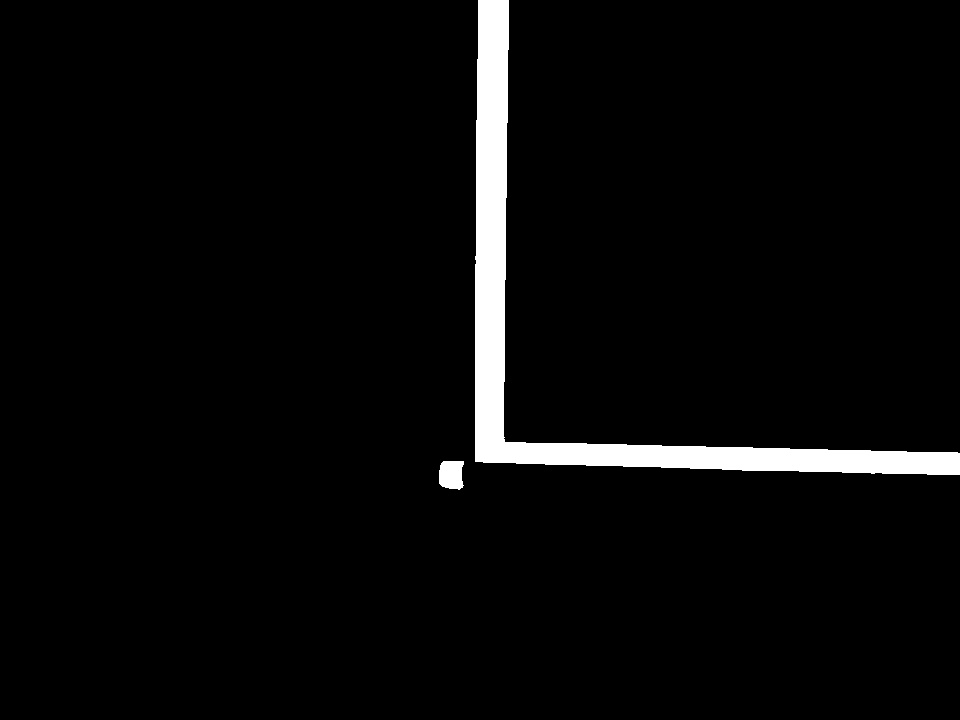
\includegraphics[width=0.7\textwidth]{picture.jpg}
		\centering
		\caption{Snapshot from the drone after initial processing - black line detected, colors inverted}
	\end{figure} 
	
	After this procedure, the snapshot is divided into 9 parts, as displayed on  figure \ref{panes}. Then, an average value of light is taken from each sub-zone. The rest of application is a state machine and its behavior depends on stage of the detection. The main state machine consists of four states:
	\begin{enumerate}
		\item sure the target zone (center) contains enough light to assume the drone is following a line,
		\item for a line to follow on the top-target, bottom-target, left-target and right-target zones,
		\item attempt to follow the llne until there is no line left.	
	\end{enumerate}
	
	The state machine is defined using an \verb|Enum|.
	
	\begin{lstlisting}
class DroneState(Enum):
	DetectCenter = 0
	DetectNextLine = 1
	FollowLine = 2
\end{lstlisting}

	\begin{figure}[h]
		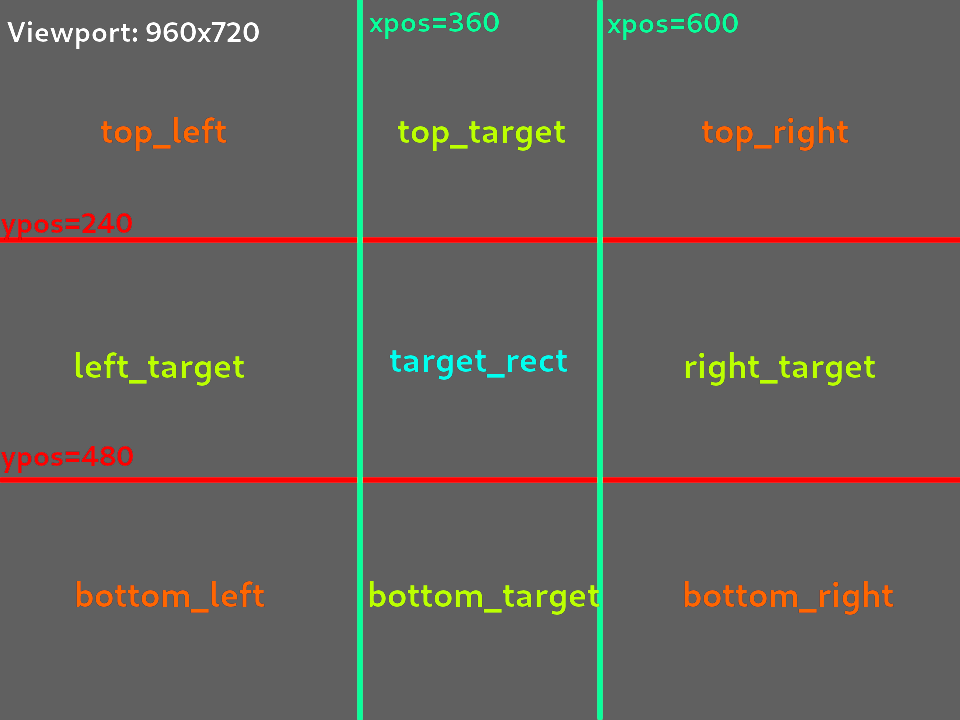
\includegraphics[width=0.8\textwidth]{split.png}
		\centering
		\caption{Tello video feed splitting for tracking}
		\label{panes}
	\end{figure}

	\begin{figure}[p]
		\includegraphics[width=0.5\textwidth]{state.pdf}
		\centering
		\caption{State machine diagram}
		\label{graph}
	\end{figure}
	
	\begin{figure}[p]
		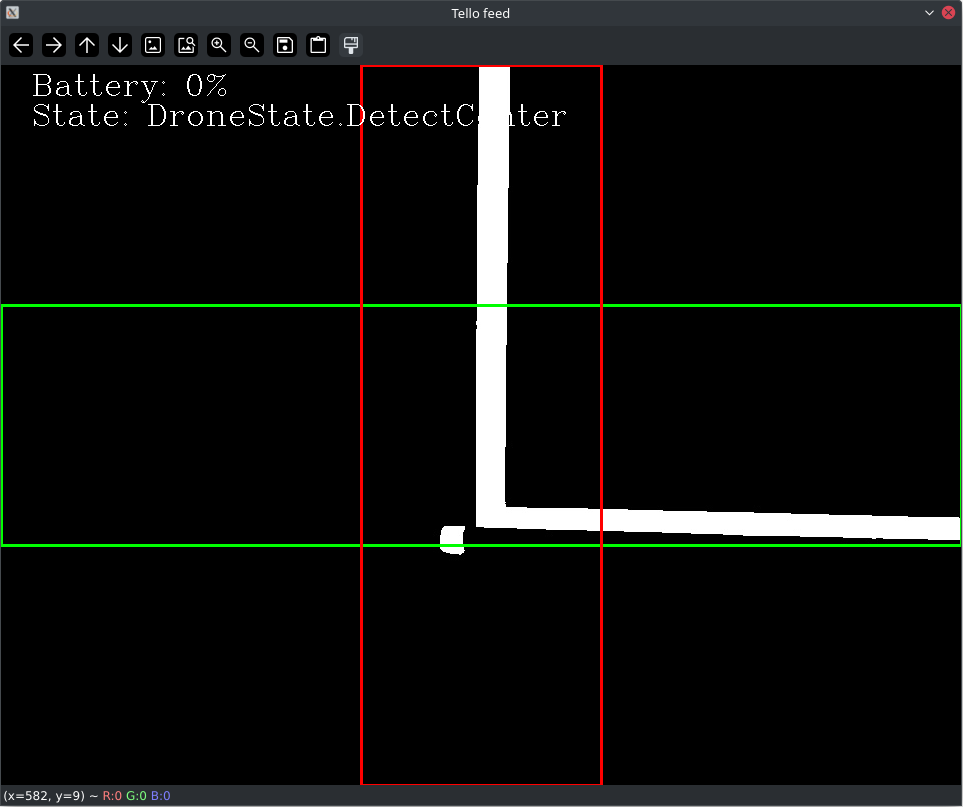
\includegraphics[width=0.8\textwidth]{demo.png}
		\centering
		\caption{UI of the application, presenting HUD and detect zones}
		\label{demo}
	\end{figure} 
	
	Afterwards, the algorithm procedes to look for a possible target to move towards, judging on the average light levels in those zones:
	\begin{itemize}
		\item in \verb|DetectCenter| state the drone moves towards any of the target zones until brightness level in \verb|target_rect| zone exceeds set threshold,
		\item in \verb|DetectLine| the drone attempts to find a possible line to follow along,
		\item in \verb|FollowLine| the drone attempts to follow the line in the area detected in \verb|DetectLine| state, until it cannot find a line anymore.
	\end{itemize}
	This relation is summarized in figure \ref{graph}. \\
	
	The algorithm's nature also has a side effect on directions the drone can travel:
	\begin{itemize}
		\item in \verb|DetectCenter| the drone can move up, down, left, right and diagonally,
		\item in \verb|DetectLine| the drone is not allowed to move and only attempts to find a direction in which a line exists,
		\item in \verb|FollowLine| the drone can only follow a direction determined in previous state.
	\end{itemize}
	
	The drone attempts to follow a line until the program is terminated, by using \verb|Space| button commanding the drone to land. \\
	
	In last stages, the program draws the rest of the HUD to the copy of original image, and displays it in a window. This stage adds a battery meter and current state onto the frame. The loop continues indefinetely.
	
	\section{Source code}
	Source code is available at GitHub: \href{https://github.com/mattroot/DjiTelloPySample}{DjiTelloPySample}. The entire source code, including this document, is licensed under the GNU General Public License version 3.0.
	
\end{document}